\chapter{INTRODUÇÃO}\label{cap:introducao}

Sistemas de segmentação de imagens têm se tornado populares em
variadas aplicações, como, por exemplo, a área de edição de imagem,
diagnósticos médicos~\cite{zhou2019interactive} e parte da visão
computacional necessária pra reconhecimento de objetos, muito
importante para desenvolvimento de direção autônoma em
carros~\cite{feng2021review}. Entre esses motivos e outros, essa área
tem uma relevância científica alta considerando a situação social,
tecnológica e econômica que é vivida no século XXI.\@

A segmentação de uma imagem pode ser feita manualmente por um anotador
humano marcando as linhas delineadoras de um objeto. Por outro lado,
são conhecidos algoritmos variados para segmentação de imagens baseados
em aprendizagem de máquina, que através de exemplos de segmentação
fornecidos para treinamento é possível inferir a segmentação de novas imagens.

Na Figura~\ref{fig:image-segmentation-types} é apresentado um quadro
comparativo de operações em uma imagem com balões, incluindo os tipos
de segmentação de imagens conhecidos: semântica e instância. Na
segmentação semântica o objetivo é segmentar apenas os mesmos tipos de
objetos como o mesmo rótulo, na segmentação por instância, cada balão
é visto como a mesma classe de balão mas com rótulos associados diferentes.

\begin{figure}[h!]
        \captionsetup{width=16cm}
		\Caption{\label{fig:image-segmentation-types}
Comparação de tipos de segmentação de imagem: por semântica e instância
}
		\centering
		\UFCfig{}{\fbox{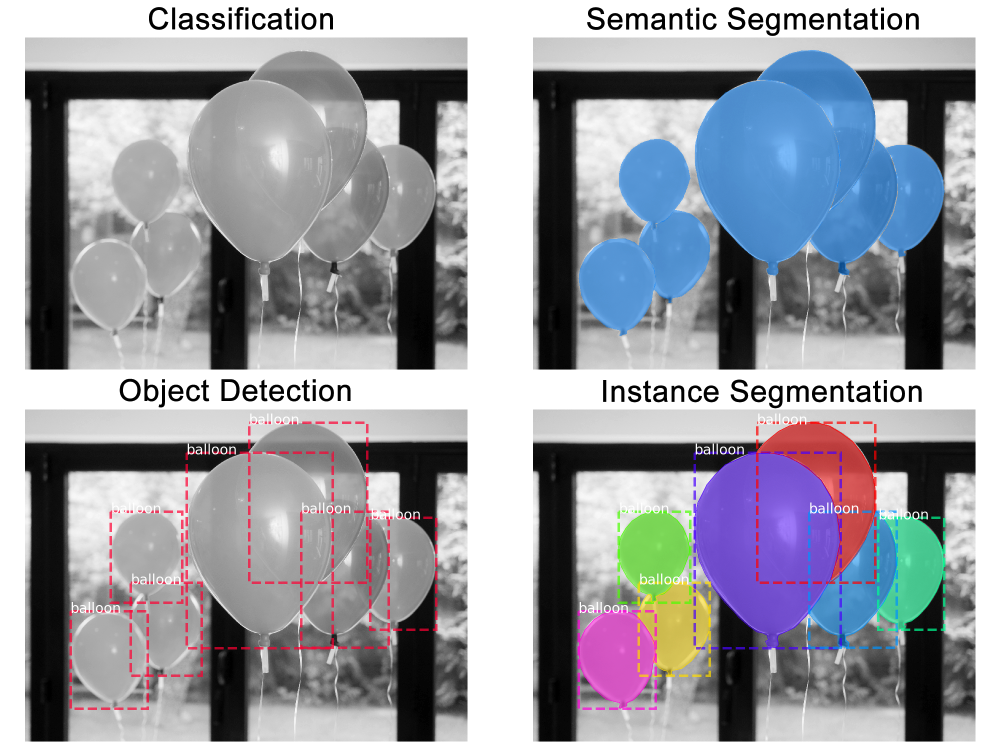
\includegraphics[width=16cm]{figuras/image-segmentation-types}}}{\Fonte{\citeonline{MediumInstanceSegmentation2019}}}
\end{figure}


Entre os tipos de aprendizagem de máquina~\cite{sah2020machine}, para segmentação de imagens
semântica é selecionada neste trabalho especificamente a aprendizagem
semi-supervisionada transdutiva\footnote{mais informações na
seção~\ref{sec:teorica-aprendizado-semi-supervisionado}}. A
aprendizagem semi-supervisionada é uma categoria que realiza o
aprendizado com poucas rotulações e a maior parte dos dados não são
rotulados. Outras categorias de aprendizado de máquina como
supervisionada possui no treinamento uma base totalmente rotulada
enquanto a aprendizagem não supervisionada não possui rótulo algum
(exemplo: K-means). Ao considerar a dificuldade de conseguir dados
rotulados por humanos em ambientes de uso por especialistas, como imagens
médicas e ferramentas de edição de imagem, a abordagem
semi-supervisionada se demonstra interessante por precisar de poucos
dados rotulados, mas ainda existir uma anotação com viés do
especialista interessado (médico, editor).


Os três principais algoritmos clássicos de segmentação de imagem podem
ser citados: \textit{Region-Based Segmentation}; \textit{Edge Detection
  Segmentation}; \textit{Segmentation based on Clustering}
~\cite{ImageSegmentationTechniques1985}. Cada uma dessas técnicas
possui limitações conhecidas, e entre elas é possível mencionar: haver
muitos objetos na imagem pode dificultar a segmentação; tempo
computacional elevado; sensibilidade ao contraste em escala cinza.

Um cenário especial de segmentação semântica abordado neste trabalho
para aplicação de um esquema de aprendizagem semi-supervisionada é o
problema de segmentação interativa\footnote{conceito explicado em
detalhes na seção~\ref{sec:segmentacao-interativa}}, no qual o
objetivo é uma segmentação binária que busca segmentar um objeto alvo
em relação ao plano de fundo. Para segmentação interativa existem
variadas técnicas, com diferentes abordagens, limitações e
vantagens~\cite{ramadan2020survey}.

Considerando tal situação-problema, este trabalho propõe a construção
de uma técnica de segmentação de imagem semi-supervisionada voltada
para segmentação interativa utilizando redes complexas e dinâmicas
coletivas de tal maneira que possa se equiparar com as melhores técnicas
atuais de segmentação interativa baseado em grafos.

\section{Trabalhos relacionados}\label{cap:trabalhos-relacionados}

Técnicas de segmentação de imagens com o paradigma semi-supervisionado
estão em foco atualmente no campo médico, como pode ser visto em
~\cite{LuoSemiSupervised2021}. Nesse artigo, uma das grandes
motivações de os autores utilizarem uma técnica semi-supervisionada
está relacionado com a dificuldade de possuir dados anotados de dados
em um domínio de dados, como imagens hospitalares.

Em relação ao tópico de redes complexas e dinâmicas coletivas, é
possível mencionar o trabalho feito com o algoritmo \gls{LCU}
~\cite{VerriNetworkUnfoldingMap2018} no qual os principais conceitos
sobre resolução de problemas de aprendizagem de máquina
semi-supervisionada são explorados em detalhes como uma dinâmica de
competição de partículas na relação vértice-arestas de um grafo
não-direcionado. Este método de aprendizagem é transdutivo, portanto,
difere dos métodos indutivos que estimam uma função de inferência no
treinamento, como é o caso de Redes Neurais. Além disso, esse
algoritmo tem complexidade computacional linear em relação à
quantidade de classes, arestas e vértices.

Para ilustrar uma possível ideia de segmentação de imagens, ao
considerar um algoritmo que faça uma transformação do domínio de
imagem para um grafo, é possível estabelecer uma relação na qual os
vértices representam parte da imagem como um \textit{superpixel}
~\cite{SuperpixelSurvey2020}, ou seja, um grupo de subpixels da
imagem. Na Figura~\ref{fig:segmentation-superpixel} é apresentado um
exemplo de segmentação usando superpixels. Algoritmos de superpixel
são não supervisionados em geral, portanto possuem suas limitações
quanto ao resultado esperado pelo usuário \textendash\hfill logo
difícil de ser aceito em aplicações médicas nas quais a opinião do
especialista é de alta relevância para o resultado final.

\begin{figure}[!h]
        \captionsetup{width=9cm}
		\Caption{\label{fig:segmentation-superpixel}
          Segmentação superpixel}
		\centering
		\UFCfig{}{
			\fbox{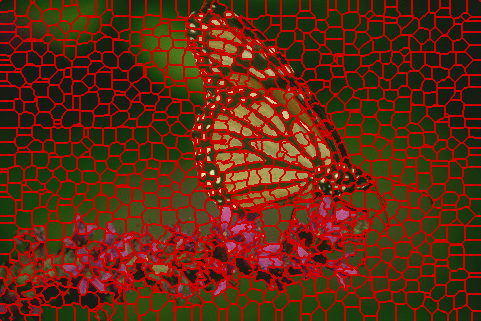
\includegraphics[width=9cm]{figuras/example-superpixel-segmentation}}
		}{
			\Fonte{\cite{SuperPixelBenchmark2017}}
		}
\end{figure}



Seguindo essa perspectiva, ao utilizar um algoritmo de extração de
\textit{features} de imagens sobre o superpixel, tem-se que o vértice
do grafo é neste momento um vetor de características. O sistema de
competição proposto no artigo \textit{Network Unfolding Map By
Vertex-Edge Dynamics Modeling}~\cite{VerriNetworkUnfoldingMap2018} pode otimizar o pertencimento de
classes (segmentos, nesse caso) baseado na topologia de sua vizinhança
e na relação aos vértices conectados. A métrica de similaridade
(por exemplo, distância euclidiana, cosseno, etc.) pode ser
ajustada de acordo com o problema.

Ao considerar o problema como semi-supervisionado, a pista de ter
alguns dos superpixels anotados adicionaria um \textit{bias}
parametrizado pelo conhecimento do especialista em uso da ferramenta,
como um editor ou um médico. A otimização do pertencimento das classes
então seria acionada pela dinâmica coletiva selecionada em questão,
que, por acaso, poderia ser o algoritmo \gls{LCU} mencionado anteriormente.

Por outro lado, ainda há muitas melhorias a serem feitas nessas técnicas, como,
por exemplo: analisar as condições de convergência do algoritmo. Isso
pode ser um dos resultados deste trabalho, demandando uma análise
matemática com auxílio de experimentos.

É importante mencionar que já foi demonstrado em outras situações,
como em~\cite{JarbasComplexNetworks2020}, que o uso de redes complexas
em fusão com redes neurais aleatórias pode gerar um discriminante de
textura da imagem de alta relevância como extrator de
características. Neste caso, é possível se apoiar nesse resultado como
uma evidência de que a investigação de novas técnicas considerando a
topologia da imagem através de redes complexas é uma oportunidade de
pesquisa.


\subsection{GrabCut: Interactive Foreground Extraction Using Iterated
  Graph Cuts}\label{sec:grabcut}

Neste trabalho, um dos pioneiros em segmentação interativa, os
autores~\cite{rother2004grabcut} desenvolveram uma técnica para segmentação interativa
chamada GrabCut baseado em um mapeamento da imagem como um grafo e
então um corte entre as arestas é realizado para segmentar o objeto do
plano de fundo.


\subsection{Aplicação de agrupamento semi-supervisionado para segmentação
  de imagens coloridas}\label{sec:franciscolira2018}

Neste trabalho, o autor~\cite{franciscolira2018}, na sua tese de
graduação, propõe variações de um algoritmo de segmentação de imagem
semi-supervisionado combinando algoritmos de agrupamento, como
\textit{Fuzzy C-Means}, Algoritmo de Pedrycs, Algoritmo
Semi-supervisionado Padrão (sSSC) e Algoritmo Semi-supervisionado
Regularizado por Entropia (ESSC).

\subsection{FocalClick: Towards Practical Interactive Image Segmentation}\label{sec:focalclick}

Neste trabalho, os autores~\cite{chen2022focalclick} criam uma técnica de
segmentação interativa em busca da praticidade, ao medir dois aspectos
importantes além de qualidade de segmentação: necessidade de anotação
e tempo de execução. O trabalho em sua metodologia de avaliação
utiliza métricas para minimizar interações que os usuários tenham que
fazer para alcançar uma segmentação de qualidade. Essa técnica se
baseia num algoritmo iterativo que possui capacidades de correção ao
incluir novas marcações. Na Figura~\ref{fig:focalclick} é possível visualizar uma
visão geral da técnica:


\begin{figure}[!h]
        \captionsetup{width=12cm}
		\Caption{\label{fig:focalclick}
          Visão geral da técnica de segmentação interativa FocalClick.}
		\centering
		\UFCfig{}{
			\fbox{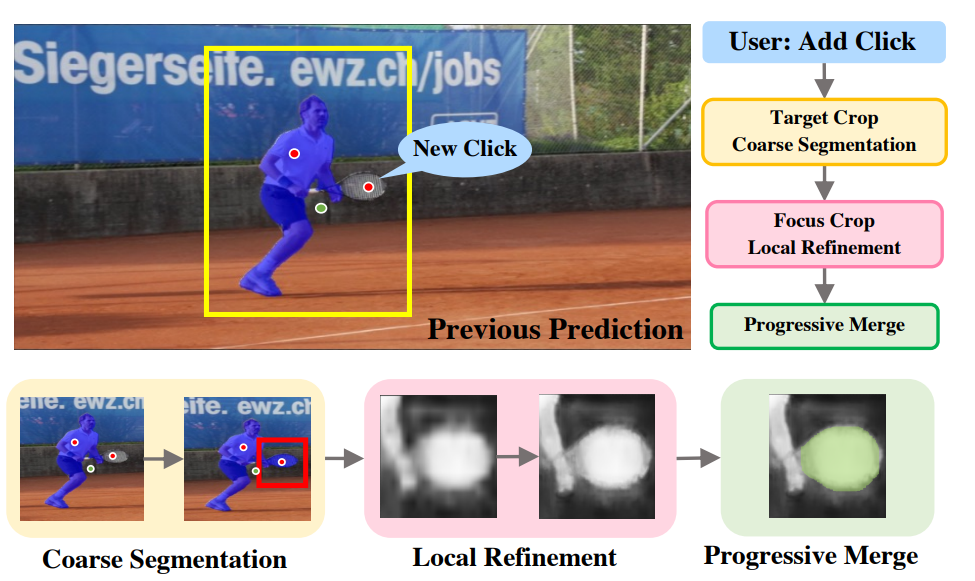
\includegraphics[width=12cm]{figuras/focalclick}}
		}{
			\Fonte{\cite{chen2022focalclick}}
		}
\end{figure}


\subsection{Interactive image segmentation based on multi-layer
random forest classifiers}\label{sec:superpixel-random-forest}

Neste trabalho, as autoras~\cite{shan2023interactive} criam uma nova
técnica para segmentação interativa de imagens combinando uma
pré-segmentação usando superpixels e duas camadas de modelos
\textit{random forest} para classificar o agrupamento entre os
superpixels numa máscara de segmentação resultante.


\section{Justificativas}\label{sec:justificativas}

Como mencionado na introdução, os algoritmos conhecidos de segmentação
de imagens possuem restrições pertinentes que podem dificultar o uso
das técnicas em alguns problemas, como imagens médicas e edição de
imagens.

Estes problemas são endereçados no desenvolvimento de uma nova técnica
de segmentação de imagens que explora outros novos ramos de
aprendizagem de máquina semi-supervisionada além das \gls{DNN}, neste
caso utilizando redes complexas e dinâmicas coletivas.

O campo de pesquisa de segmentação interativa também tem tido aumento
na publicação de artigos de relevância, em especial a publicação de
artigos com a palavra-chave GrabCut (tipo de algoritmo para
segmentação interativa), como pode ser visto na
Figura~\ref{fig:grabcut-papers}:

\begin{figure}[!h]
        \captionsetup{width=12cm}
		\Caption{\label{fig:grabcut-papers}
          Quantidade de publicações relevantes envolvendo grabcut de
          2004 a 2022}
		\centering
		\UFCfig{}{
			\fbox{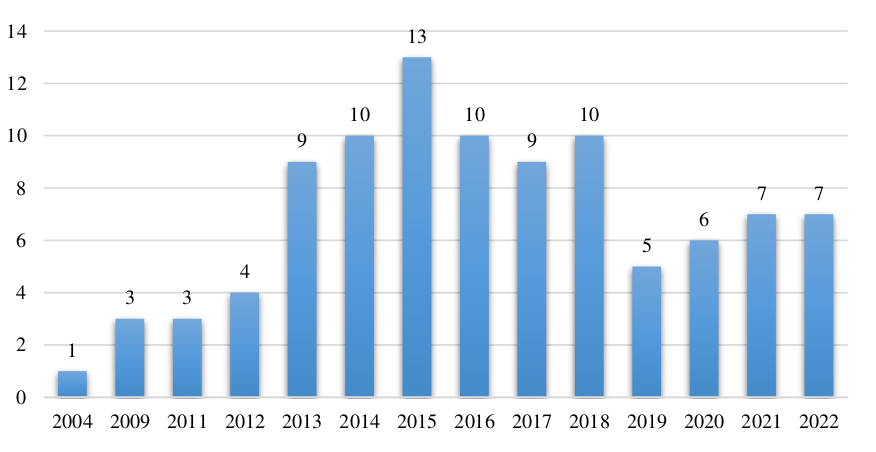
\includegraphics[width=12cm]{figuras/grabcut-papers}}
		}{
			\Fonte{\cite{wang2023review}}
		}
\end{figure}



\section{Objetivo Geral}\label{sec:objetivo-geral}

Desenvolver uma nova técnica de segmentação de imagens
semi-supervisionada que possa ser equiparável ao estado da arte, com
foco em segmentação interativa.

\section{Objetivos Específicos}\label{sec:objetivo-geral}

\begin{itemize}
\item Explorar técnicas de redes complexas e dinâmicas coletivas sobre
  o problema de segmentação de imagens.
\item Aplicar em casos variados de segmentação de imagens, como
  objetos comuns, carros.
\item Avaliar o impacto da segmentação por superpixel na segmentação final.
\item Desenvolver uma ferramenta para segmentação interativa
  utilizando o método de segmentação proposto.
\end{itemize}



% LocalWords:  transdutivo superpixel
